\documentclass[aspectratio=169,10pt]{beamer}

\usepackage[utf8]{inputenc}

\usepackage{multicol}
\usepackage{multirow}
\usepackage{textcomp} % to use \textmu
\usepackage[absolute,overlay]{textpos} % to place floating text boxes with \begin{textblock*}{width}(x,y)
\usepackage{tcolorbox}

\usepackage{tikz}
\usetikzlibrary{decorations.pathreplacing}

\usepackage{graphicx}
\graphicspath{{./figuras/}}

\setbeamertemplate{navigation symbols}{}

\title[Flujo de Back-End]{El Flujo de Diseño Analógico}
\subtitle{Back-End}
\author[Dr.-Ing. Juan José Montero-Rodríguez]{Dr.-Ing. Juan José Montero-Rodríguez}
\institute[]{Instituto Tecnológico de Costa Rica\\Escuela de Ingeniería Electrónica\\Elementos Activos}
\date{Semestre I-2019}
\titlegraphic{
\includegraphics[height=8mm]{logoTEC.png}}


\begin{document}

\begin{frame}
\titlepage
\end{frame}


\begin{frame}[t]
\frametitle{Objetivos}

\textbf{Principios de fabricación de circuitos integrados (2.5 semanas)}

\begin{itemize}
\item El proceso de fabricación CMOS: materiales, técnicas y flujo de fabricación, prevención de efecto de enganche
\item Integración de elementos pasivos, capacitores conmutados para integración de resistencias.
\item Principios de layout e introducción al flujo de back-end
\end{itemize}

Objetivos

\begin{itemize}
\item Conocer los principios de fabricación de circuitos integrados CMOS
\item Aplicar técnicas básicas de layout y principios básicos del flujo backend
\end{itemize}
\end{frame}


\begin{frame}
\frametitle{El Flujo de Diseño Analógico}
\centering
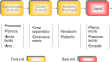
\includegraphics[width=11cm]{flujo1}
\end{frame}


\begin{frame}
\frametitle{El Flujo de Diseño Analógico}
\centering
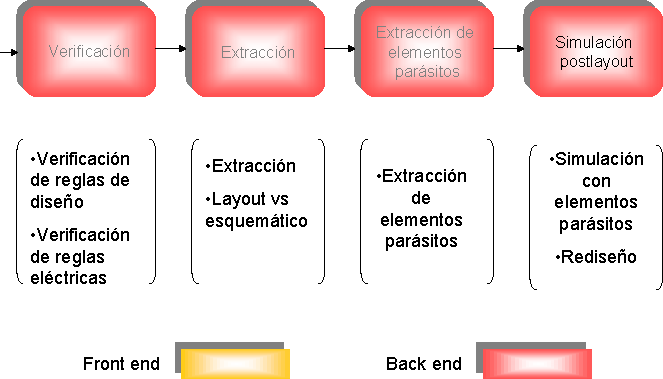
\includegraphics[width=11cm]{flujo2}
\end{frame}


\begin{frame}[t]
\frametitle{Flujo de Back-End}

\begin{itemize}
\item Back-end: diseño físico y verificación del diseño después del diseño físico
\item Incluye una serie de verificaciones para asegurar fabricación exitosa:
\begin{itemize}
\item Verificación de reglas de diseño (DRC)
\item Verificación de layout contra esquemático (LVS)
\item Extracción de elementos parásitos
\item Simulación de postlayout
\item Puede incluir también verificación de reglas eléctricas (ERC) y de errores de antena
\end{itemize}
\end{itemize}
\end{frame}


\begin{frame}[t]
\frametitle{Layout}
\begin{columns}
	\begin{column}{0.5\textwidth}
		\begin{itemize}
			\item Layout: representación geométrica de los componentes a integrar y sus interconexiones
			\item Los componentes se representan con diferentes colores y polígonos
			\begin{itemize}
				\item Colores representan materiales y propiedades
				\item Polígonos representan la forma en la que se debe moldear una capa durante la fabricación = forma final que debe tener la capa
			\end{itemize}
			\item El layout se utiliza para obtener la información para fabricar las máscaras
			\item Debe cumplir las reglas de diseño del fabricante
		\end{itemize}
	\end{column}
	\begin{column}{0.5\textwidth}
		\centering
		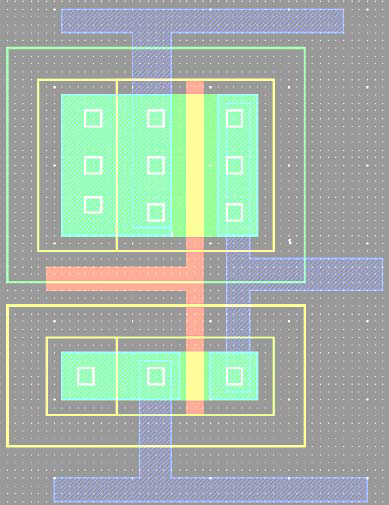
\includegraphics[width=5cm]{layout}
	\end{column}
\end{columns}
\end{frame}


\begin{frame}[t]
\frametitle{Reglas de Diseño}
\begin{itemize}
	\item Define geometría permitida y relaciones geométricas permitidas en el proceso de fabricación
\end{itemize}

\begin{columns}
	\begin{column}{0.4\textwidth}
	\begin{itemize}
		\item Reglas definidas por las características del proceso de fabricación
		\item Deben respetarse para asegurar que el chip sea fabricado correctamente
	\end{itemize}
	
	\centering
	\vspace{3mm}
	$\Downarrow$
	\vspace{3mm}
	\begin{tcolorbox}[colframe=red,colback=white]
		\centering
		Verificación de reglas de diseño
		
		(DRC, design rules check)
	\end{tcolorbox}
	\end{column}
	\begin{column}{0.6\textwidth}
		\centering
		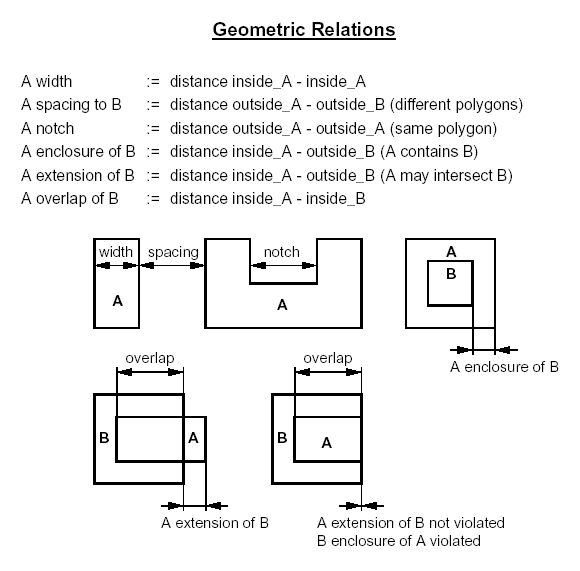
\includegraphics[width=7cm]{DRC}
	\end{column}
\end{columns}
\end{frame}


\begin{frame}[t]
\frametitle{Reglas de Diseño}
Reglas de diseño incluyen restricciones de 4 tipos:

\begin{itemize}
\item Ancho: precisión de litografía y de otros pasos de fabricación define el ancho (y largo) mínimo de un polígono
\item Espaciamiento: fabricación impone restricciones de espaciamiento entre estructuras. Ej: evita corto circuitos y efectos de enganche
\item Encapsulamiento: distancia mínima de traslape entre una estructura interna y otra que debe rodearla: Ej: contactos deben estar rodeados de metal para asegurar contacto eléctrico entre las capas por conectar
\item Extensión: algunas estructuras deben extenderse más allá del borde de otras estructuras. Ej: compuerta de polisilicio debe extenderse más allá de las regiones de difusión a su lado
\end{itemize}
\end{frame}


\begin{frame}[t]
\frametitle{Extracción}
\begin{itemize}
	\item Extracción:
	\begin{itemize}
		\item Los polígonos del layout deben interpretarse para verificar que los componentes y conexiones fueron representados correctamente
		\item Permite conocer el impacto de elementos parásitos: resistencias y capacitancias parásitas, diodos parásitos
		\item Información requerida para creación de máscaras
	\end{itemize}
	\item Existen herramientas de software para la extracción
	\begin{itemize}
		\item Requieren dibujo de capas físicas
		\item Requieren dibujo de capas auxiliares para la interpretación de los componentes representados = capas lógicas
	\end{itemize}
	\item Dos tipos de capas:
	\begin{itemize}
		\item De máscara
		\item Lógicas (de definición)	
	\end{itemize}
\end{itemize}
\end{frame}


\begin{frame}[t]
\frametitle{Capas de Máscara}
Capas con las cuales se fabrican las máscaras para fabricar el circuito integrado

\centering
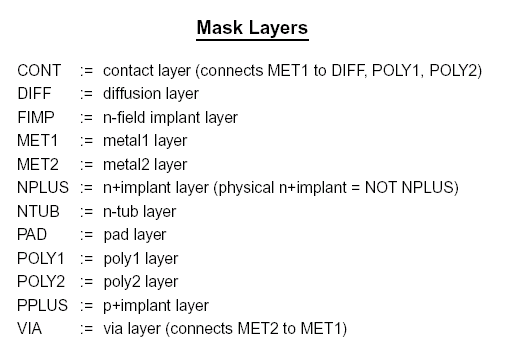
\includegraphics[width=10cm]{masks}
\end{frame}


\begin{frame}[t]
\frametitle{Capas de Definición}
Capas lógicas, es decir, son una ayuda para la herramienta de extracción y verificación; no se utilizan en durante el proceso de fabricación del chip

\centering
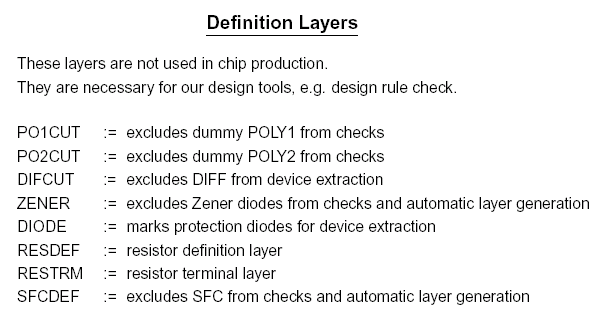
\includegraphics[width=11.5cm]{deflayers}
\end{frame}


\begin{frame}[t]
\frametitle{Definición de Estructuras}
Ejemplo de definición de estructuras para la extracción

\centering
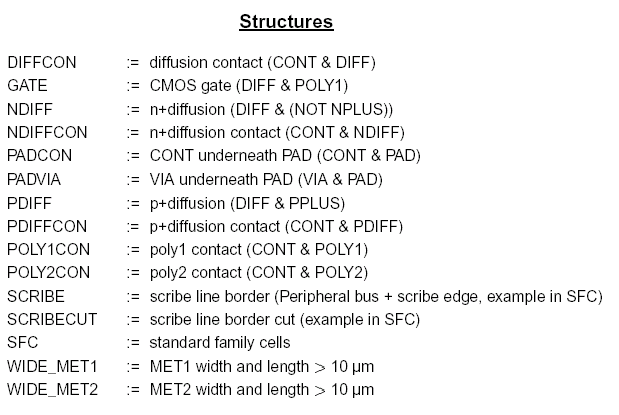
\includegraphics[width=10cm]{structures}
\end{frame}


\begin{frame}[t]
\frametitle{Definición de Componentes}
La definición de estructuras depende de los componentes que pueden fabricarse en el proceso

\centering
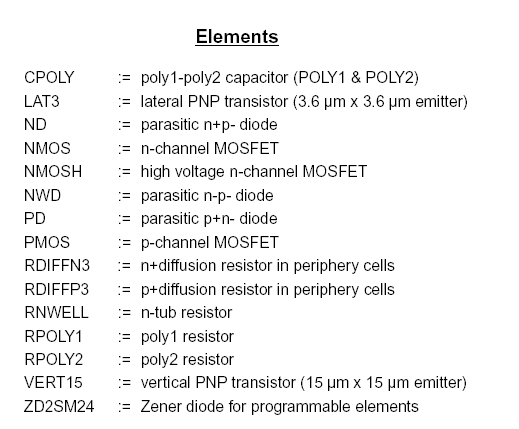
\includegraphics[width=8cm]{components}
\end{frame}


\begin{frame}[t]
\frametitle{Reglas de Extracción}
La extracción se basa en la intersección de polígonos de diferentes capas

\vspace{3mm}
Las intersecciones requeridas para cada componente se definen por medio de reglas de extracción dadas por el fabricante

\vspace{3mm}
\centering
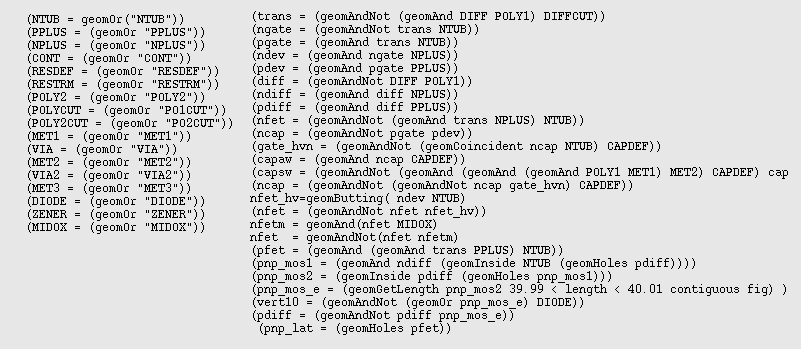
\includegraphics[width=12cm]{extraction}
\end{frame}


\begin{frame}[t]
\frametitle{Layout vs Esquemático}
\begin{itemize}
\item Una vez interpretado el layout (extraído), debe verificarse que los componentes y conexiones presentes representan el circuito que se diseñó en el esquemático
\item Esta verificación se conoce como LVS (layout versus esquemático)
\item Se revisa cada componente, así como sus interconexiones
\end{itemize}

\centering
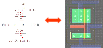
\includegraphics[width=11cm]{LVS}
\end{frame}



\begin{frame}[t]
\frametitle{Simulación de Postlayout}
\begin{itemize}
\item Los elementos parásitos presentes y su magnitud sólo pueden saberse después de finalizar el layout
\item En las primeras simulaciones, no se tomaron en cuenta estos elementos
\item Simulación de postlayout:
\begin{itemize}
	\item Verificación de características y funcionalidad del circuito tomando en cuenta los elementos parásitos
\end{itemize}
\item Elementos parásitos pueden afectar el funcionamiento del circuito $\Rightarrow$ puede requerir rediseño completo
\end{itemize}
\end{frame}



\begin{frame}[t]
\frametitle{Sección Transversal de un Inversor CMOS}
\centering
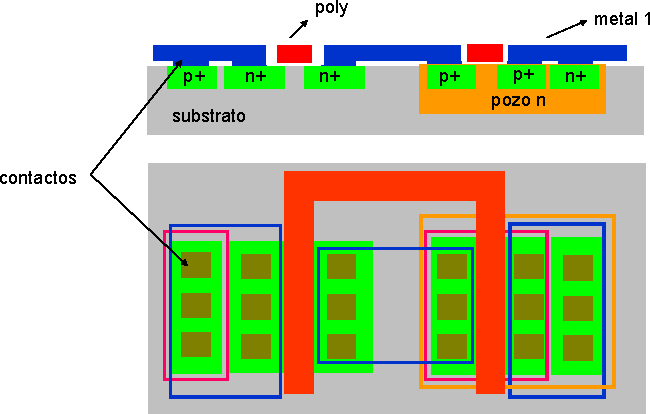
\includegraphics[width=11cm]{CMOSa}
\end{frame}


\begin{frame}[t]
\frametitle{Layout vs Sección Transversal}
\centering
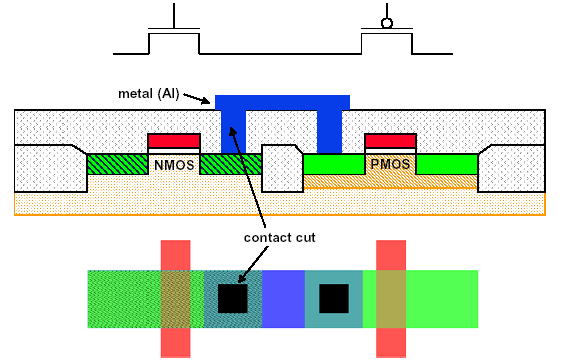
\includegraphics[width=11cm]{CMOSb}
\end{frame}


\begin{frame}[t]
\frametitle{Layout vs Sección Transversal}
\centering
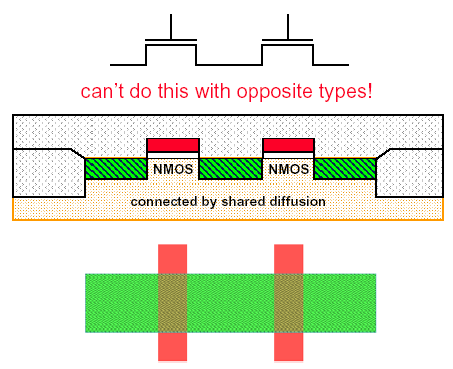
\includegraphics[width=9cm]{CMOSc}
\end{frame}


\begin{frame}[t]
\frametitle{Layout vs Sección Transversal}
\centering
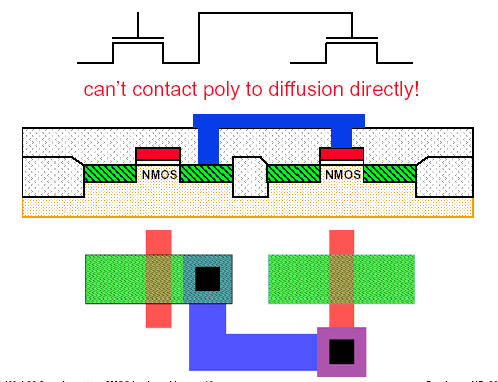
\includegraphics[width=9cm]{CMOSd}
\end{frame}


\begin{frame}[t]
\frametitle{Layout de Inversor}
\centering
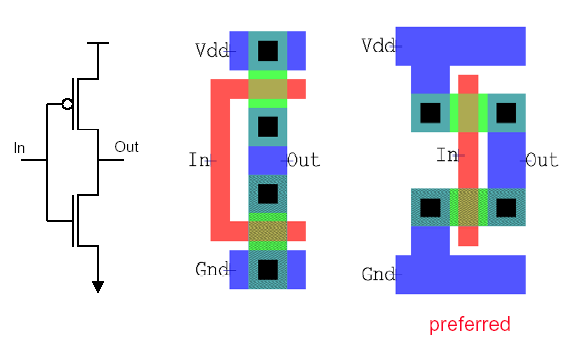
\includegraphics[width=12cm]{inverter}
\end{frame}


\begin{frame}[t]
\frametitle{Ejemplo de Layout con Proceso Comercial}
\centering
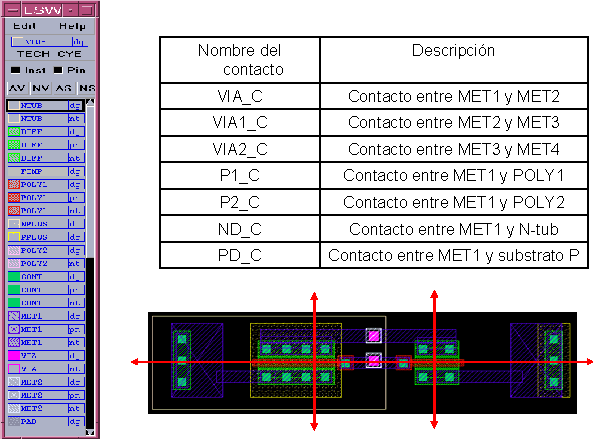
\includegraphics[width=10cm]{layout2}
\end{frame}


\begin{frame}[t]
\frametitle{Errores de Antena}
\centering
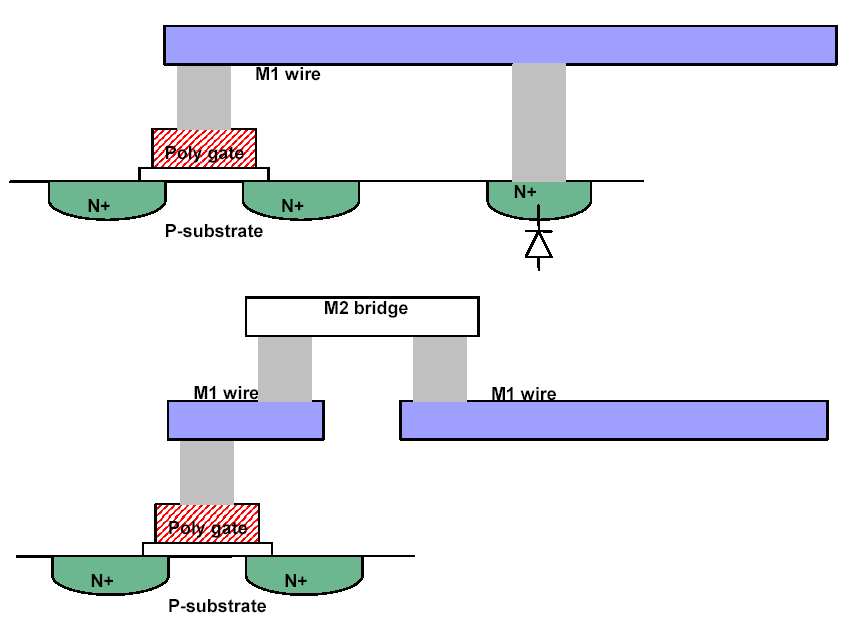
\includegraphics[width=10cm]{antenna}
\end{frame}


\begin{frame}[t]
\frametitle{Integración de Resistencias}
\begin{columns}
\begin{column}{0.2\textwidth}
	Métodos:
\end{column}
\begin{column}{0.8\textwidth}
	\begin{itemize}
		\item Interconexión de silicio policristalino dopado
		\item Regiones de difusión
	\end{itemize}
\end{column}
\end{columns}

\vspace{3mm}
\begin{columns}
	\begin{column}{0.2\textwidth}
		\[ R = \dfrac{\rho L}{Wt} \]
	\end{column}
	\begin{column}{0.8\textwidth}
		L: longitud de interconexión
		
		t: espesor de interconexión
		
		W: ancho de interconexión
	\end{column}
\end{columns}


\vspace{5mm}\centering

\includegraphics[width=6cm]{resist}

\raggedright
\vspace{5mm}
Espesor de conductor es definida por el proceso

\vspace{3mm}
Resistencias integradas presentan una tolerancia de $\pm$20\% (precisión de la litografía, decapado y difusión, además de variaciones en el espesor la interconexión)
\end{frame}


\begin{frame}[t]
\frametitle{Integración de Resistencias}
"Serpentinas" se usan para obtener resistencias de mayor valor en una estructura compacta

\centering\vspace{5mm}
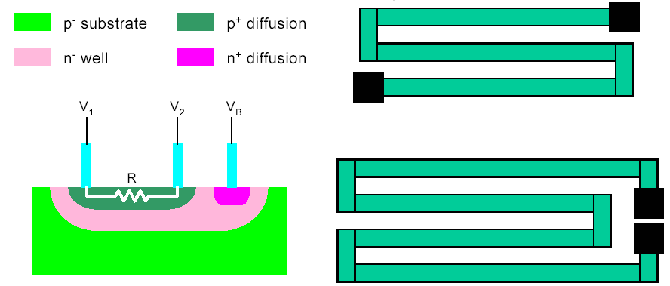
\includegraphics[width=13cm]{resist2}
\end{frame}


\begin{frame}[t]
\frametitle{Capacitores Conmutados}
Permiten emular resistencias de gran valor ocupando un área de fabricación menor (ej: 1 M$\Omega$)

\centering\vspace{5mm}
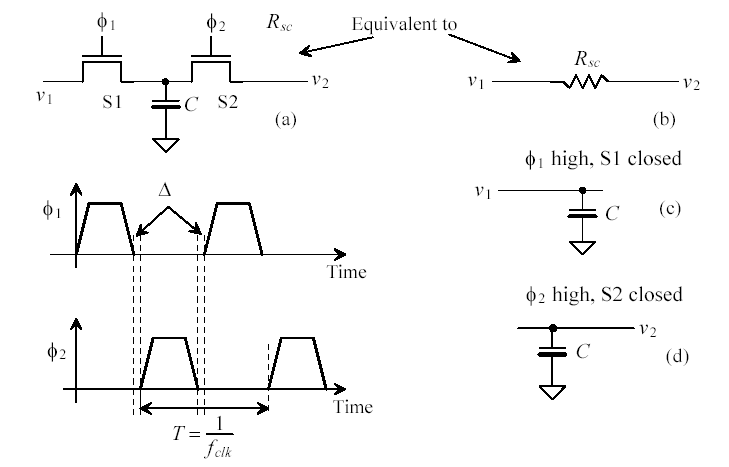
\includegraphics[width=10cm]{swcap}
\end{frame}


\begin{frame}[t]
\frametitle{Capacitores Conmutados}
\centering
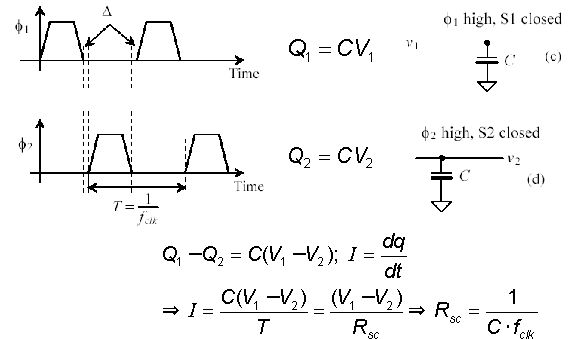
\includegraphics[width=12cm]{swcap2}
\end{frame}


\begin{frame}[t]
\frametitle{Integración de Capacitores}
\begin{itemize}
	\item Rango de capacitancia posible en fabricación: $<$ 100 pF
	\item Técnicas
	\begin{itemize}
		\item Transistor MOS: B,S y D al mismo potencial para formar una placa, G es la otra placa. Polarizado en inversión
		\item Óxido delgado sobre área de difusión fuertemente dopada y silicio policristalino o metal como placa superior
		\item Pila de primer nivel de polisilicio, óxido y segundo nivel de polisilicio
	\end{itemize}
\end{itemize}

\centering\vspace{5mm}
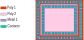
\includegraphics[width=8cm]{caps}
\end{frame}


\begin{frame}[t]
\frametitle{Ejemplo 1}
\centering
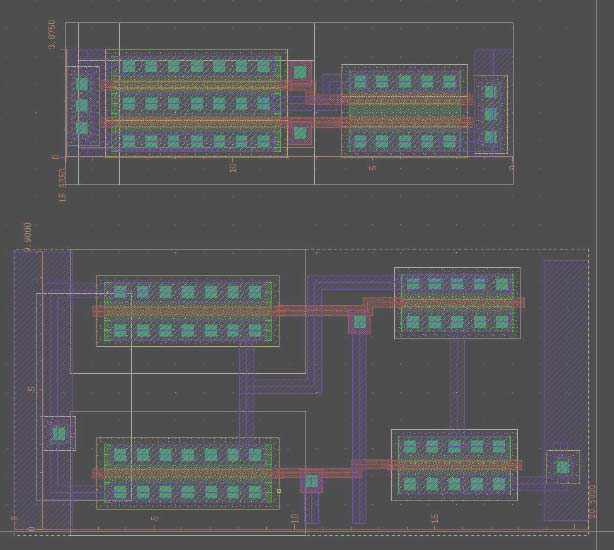
\includegraphics[width=8cm]{ejemplo}
\end{frame}


\begin{frame}[t]
\frametitle{Proceso CMOS con Componentes Pasivos}
\centering
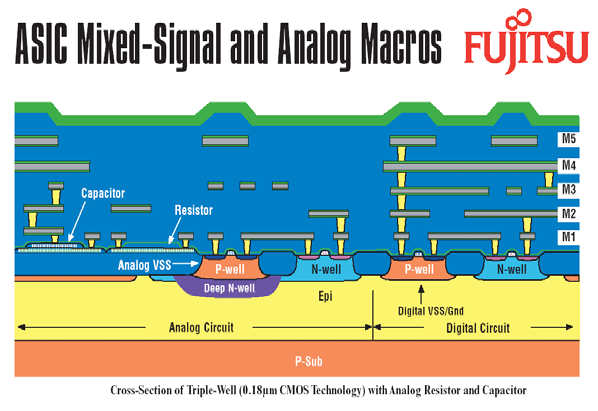
\includegraphics[width=11cm]{fujitsu}
\end{frame}

\end{document}
